\documentclass[t]{beamer}
\usepackage{pdfpages}
\usepackage{wrapfig}
\usepackage{cutwin}
\usetheme{Juelich}
\setbeamertemplate{footer element1}[logo]{arbor-lines-proto-colour}

\title{Introduction to Arbor}
\subtitle{What's new and demonstration}
\author{Brent F. B. Huisman}
\institute{Jülich Supercomputing Centre}
\date{\today}
\titlegraphic{\includegraphics%
    [width=\paperwidth]{placeholder}}

\newcommand{\lenitem}[2][.6\linewidth]{\parbox[t]{#1}{\strut #2\strut}}

\begin{document}
\maketitle

\small

\begin{frame}
    \frametitle{What is Arbor?}
    \framesubtitle{}
%     \vspace{0.5 \baselineskip}
        Arbor is a library for implementing performance portable network simulations of multi-compartment neuron models.
        % \begin{wrapfigure}{r}{20mm}
        %     \begin{center}
        %         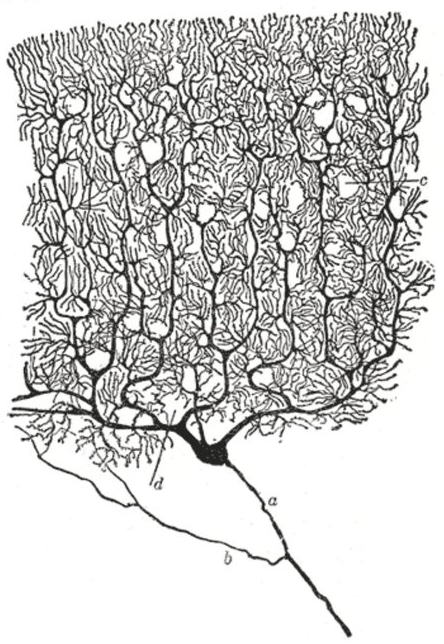
\includegraphics[width=\linewidth]{purkinje.png}
        %     \end{center}
        % \end{wrapfigure}

        \begin{itemize}
        \item Simulate large networks of morphologically-detailed, spiking neurons
        \item Library: you control your program/workflow. Interoperable.
        \item Portable: scientific description is separate from execution instructions. E.g. run one scientific description on laptop CPU, GPU cluster or future hardware.
        \item \textit{Performance} portable: add optimized backends for new computer architectures. Currently supported:
            \begin{itemize}
            \item Distributed parallelism using MPI
            \item CUDA backend for NVIDIA and AMD GPUs
            \item Vectorized backends for x86-64 (KNL, AVX, AVX2) and Arm64 (NEON, SVE) intrinsics
            \end{itemize}
        \item Executes on all HPC systems in the HBP (and outside).
        \end{itemize}
\end{frame}

\begin{frame}
    \frametitle{Who is Arbor?}
    % \framesubtitle{\url{arbor-sim.org}}

    Repo: \url{github.com/arbor-sim/arbor}, website: \url{arbor-sim.org}
    \begin{itemize}
        \item Latest release: v0.6
        \item 48 Github forks, 69 Github stars
        \item 1400+ commits to main branch
        \item loc: C++: 157k, Python: 13k, reStructuredText: 21k
        \item 26 contributors, from 9+ institutions
        % from Lugano, Zürich, Jülich, Pavia, Oslo, Göttingen, Utrecht, Heidelberg, Barcelona, and more!
    \end{itemize}

    \begin{wrapfigure}{r}{40mm}
        \begin{center}
            
\includegraphics[width=\linewidth]{cscs_logo.pdf}
        \end{center}
        \vspace{0.1\baselineskip}
        \begin{center}
            
\includegraphics[width=\linewidth]{Logo_FZJ_JSC.pdf}
        \end{center}
    \end{wrapfigure}

    Core contributors
    \begin{itemize}
        \item Ben Cumming, Nora Abi Akar,
        \item[] Fabian Bösch, Simon Frasch,
        \item[] Lukas Drescher
        \item Anne Küsters, Thorsten Hater,
        \item[] Brent Huisman
    \end{itemize}
    

\end{frame}


{
\setbeamercolor{background canvas}{bg=}
\includepdf[pages={2,6,7}]{20180929_f.huber.pdf}
}


\begin{frame}{Arbor design}
    \begin{itemize}
    \item Modular: components can be substituted according to internal API
    \item Internal API: `thin' API; type parameterization allows components to determine low-overhead API data structures
    \end{itemize}
    \begin{center}
      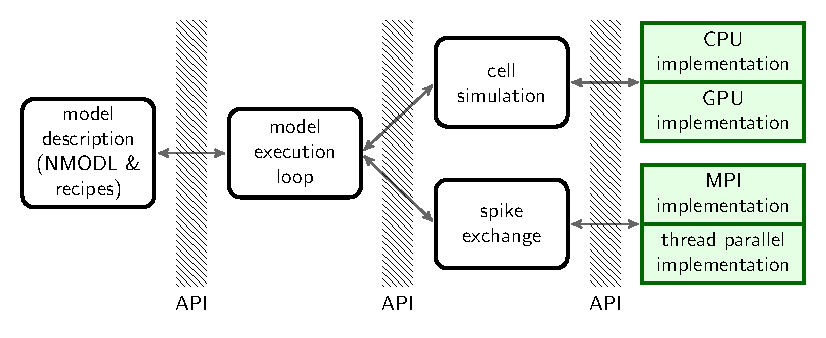
\includegraphics[width=.9\textwidth]{api.pdf}
    \end{center}
  \end{frame}
  
  
  \begin{frame}{Arbor backends}
    Cell simulation modules share computational backends for channel and synapse state evolution.
  
    \vfill
    \centering
    CPU-hosted finite volume cell simulation\\
    \vspace{2ex}
    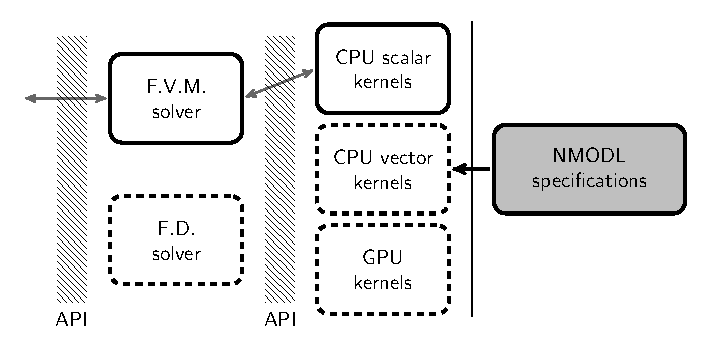
\includegraphics[height=0.5\textheight]{backend-api.pdf}
  
    \vfill
  \end{frame}
  
  \begin{frame}{Cell simulation timeloop}
    \begin{center}
      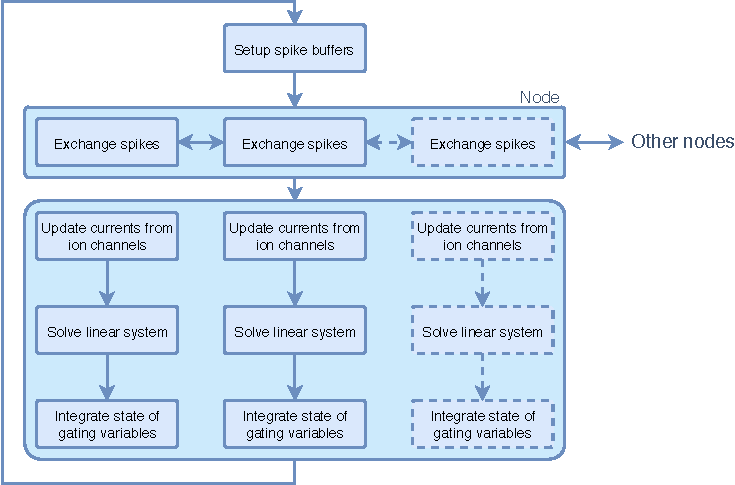
\includegraphics[height=.75\textheight]{timeloop.pdf}
    \end{center}
  \end{frame}


\begin{frame}
    \frametitle{Wrap up}
    \framesubtitle{Questions?}
    \begin{itemize}
        \item Web: \url{arbor-sim.org}
        \item Docs: \url{docs.arbor-sim.org}
        \item Community: \url{github.com/arbor-sim/arbor/discussions}
        \item Chat: \url{gitter.im/arbor-sim/community}
        \item[]
    \end{itemize}

    { \scriptsize Acknowledgements: This research has received funding from the European Unions
    Horizon 2020 Framework Programme for Research and
    Innovation under the Specific Grant Agreement No. 720270
    (Human Brain Project SGA1), Specific Grant Agreement No.
    785907 (Human Brain Project SGA2), and Specific Grant
    Agreement No. 945539 (Human Brain Project SGA3). }
    \newline
    \begin{figure}[h]
        \begin{center}
            
\includegraphics[width=0.2\linewidth]{ebrains_logo.png}
            \hspace{2em}
            
\includegraphics[width=0.4\linewidth]{HBP_logo.jpg}
        \end{center}
    \end{figure}
\end{frame}


\end{document}
